\documentclass{article}

\usepackage{../definition}
\usepackage{../theorem}
\usepackage{../preamble}

\title{Лекция 4}
\author{}
\date{24 сентября 2024}

\begin{document}
    \maketitle
    \noindent
    \underline{Замечание:} существование предела функции в точке никак не связано с тем, опрделена сама функция в этой точке или нет.\\
    \underline{Домашнее задание:} привести пример, когда функция в точке определена, а предела в этой точке у неё нет.    
    \begin{figure}[h]
        \begin{subfigure}[t]{0.3\textwidth}
            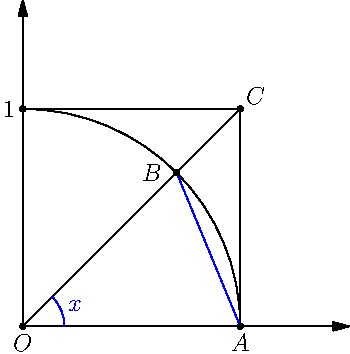
\includegraphics{pic-1.pdf}
            \caption{}
        \end{subfigure}
        \hfill
        \begin{subfigure}[t]{0.3\textwidth}
            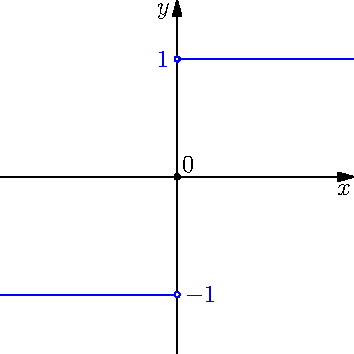
\includegraphics{pic-2.pdf}
            \caption{\(y = sign(x)\)}
        \end{subfigure}
        \hfill
        \begin{subfigure}[t]{0.3\textwidth}
            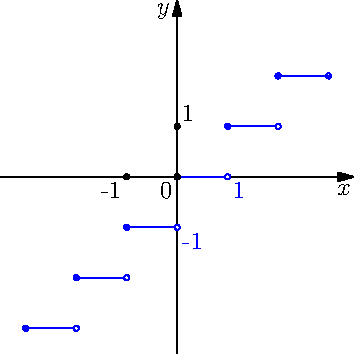
\includegraphics{pic-3.pdf}
            \caption{\(y = [x]\)}
        \end{subfigure}
    \end{figure}\\
    \textbf{Пример 6 (рисунок a).} \(f(x) = \sin(x)\). Докажем, что \(\displaystyle \lim\limits_{x \to 0}\sin(x) = 0\):
    \begin{enumerate}
        \item Площадь равнобедренного треугольника \(OAB\), вписанного в сектор единичной окружности, меньше площади этого сектора: 
        \(\displaystyle S_{AOB} = \frac{1}{2}\sin(x) < S_{\text{сект.} AOB} = \frac{1}{2}x \implies \sin(x) < x\) при \(\displaystyle 0 < x < \frac{\pi}{2}\).
        \item С другой стороны, \(\displaystyle S_{\text{сект.} AOB} < S_{AOC}\), то есть \(\displaystyle \frac{1}{2}x < \frac{1}{2} \tan(x) \iff x < \tan(x)\).
        \item В силу нечетности функций \(\sin(x)\) и \(x\): \(|\sin(x)| < |x|\).
        \item Воспользуемся определением предела: \(\displaystyle \forall \varepsilon > 0\ \exists \delta(\varepsilon) = \varepsilon > 0\ \forall x: 0 < |x| < \delta \implies |\sin(x) - 0| = |\sin(x)| < |x| < \varepsilon\).
    \end{enumerate}       
    \section{Односторонние пределы}
    Может случиться так, что при \(x \to a\) функция \(f(x)\) имеет разные предельные значения.\\
    \textbf{Пример 1 (рисункок b).} \(f(x) = sign(x) = 
    \begin{cases}
        +1 & \text{если}\ x > 0\\
        \ \ 0 & \text{если}\ x = 0\\
        -1 & \text{если}\ x < 0\\ 
    \end{cases}\).
    \begin{definition}
        Число \(B\) называется пределом функции \(f(x)\) в точке \(a\) справа, если
        \(
            \forall \varepsilon > 0\ \exists \delta > 0 : \forall x \in (a, a + \delta)\ |f(x) - B| < \varepsilon
        \).
    \end{definition}
    \noindent
    \underline{Замечание:} обозначается как \(\lim\limits_{x \to a^{+}}f(x) = B\) или \(f(a + 0) = B\).\\ 
    \textbf{Пример 2 (рисунок c).} \(f(x) = [x]\). Целая часть числа \(x\)  --- это такое наибольшее целое число, не превосходящее \(x\).
    \(f(n - 0) = n - 1\), \(f(n + 0) = n\).
    \begin{theorem}[О свзяи пределов]
        Существование предела в точке равносильно существованию равных односторонних пределов в этой точке.\\
        \[\lim\limits_{x \to a}f(x) = A \iff 
        \begin{cases}
            \lim\limits_{x \to a^{+}}f(x) = A\\
            \lim\limits_{x \to a^{-}}f(x) = A\\
        \end{cases}\]. 
    \end{theorem}   
    
    %────────────────────────────────────────────────────────────────────────────────────────────────────────────────────────────────────────────────────
    \section{Предел функции при \(x \to \infty\)}
    Пусть \(f(x)\) задана на множестве \(X\) и \(\forall A\ \exists x \in X: x > A\).
    \begin{definition}
        Число \(B\) называется педелом функции \(f(x)\) при \(x \to +\infty\), если
        \(
            \forall \varepsilon > 0\ \exists A(\varepsilon) : \forall x > A\ |f(x) - B| < \varepsilon
        \).
    \end{definition}
    \noindent
    \underline{Замечание 1:} обозначается как \(\lim\limits_{x \to +\infty}f(x) = B\).\\
    \underline{Замечание 2:} если \(
    \begin{cases}
        \lim\limits_{x \to +\infty}f(x) = B\\
        \lim\limits_{x \to -\infty}f(x) = B\\
    \end{cases}
    \), то пишут \(\lim\limits_{x \to \infty}f(x) = B\).\\
    \textbf{Пример.} \(\displaystyle f(x) = \frac{1}{x}\). Докажем, что \(\lim\limits_{x \to \infty}f(x) = 0\).
    \begin{enumerate}
        \item Зафиксируем произвольное \(\varepsilon > 0\). 
        \item Выберем в качестве \(A\) число \(\frac{1}{\varepsilon}\).
        \item Получим, что \(\displaystyle \forall x > A: |f(x) - 0| = \frac{1}{x} < \varepsilon\). 
    \end{enumerate}
    \noindent
    \underline{Замечание:} частный случай предела функции при \(x \to +\infty\) --- это предел числовой последовательности.
    
    %────────────────────────────────────────────────────────────────────────────────────────────────────────────────────────────────────────────────────
    \section{Бесконечно малые и бесконечно большие функции}
    \begin{definition}
        Функция \(f(x)\) называется бесконечно малой в точке \(a\) (при \(x \to a\)), если \(\lim\limits_{x \to a}f(x) = 0\).
    \end{definition}
    \noindent
    \underline{Домашнее задание:} записать это определение на языке \(\varepsilon\), \(\delta\).\\
    \textbf{Пример 1.} \(\displaystyle \sin(x)\) бесконечно малая в точке \(0\).\\
    \underline{Замечание:} функция бесконечно малая в точке \(a\) --- вообще говоря --- в точке \(a\) может не обращаться в 0.\\
    \textbf{Пример 2.} \(\displaystyle f(x) =
    \begin{cases}
        \sin(x) & \text{если}\ x \neq 0\\
        1 & \text{если}\ x = 0\\ 
    \end{cases}\) бесконечно малая в точке 0.\\
    \underline{Замечание:} не всякая функция, обращающаяся в 0 в точке \(a\), является бесконечно малой.\\
    \textbf{Пример 3.} \(\displaystyle f(x) = \frac{1}{x}\) бесконечно мала при \(x \to \infty\).
    \begin{definition}
        Функция \(f(x)\) называется бесконечно большой в точке \(a\) (при \(x \to a\)), если \(\forall A > 0\ \exists \delta > 0: \forall x: 0 < x < \delta \implies |f(x)| > A\).  
    \end{definition}
    \noindent
    \underline{Замечание 1:} обозначается как \(\lim\limits_{x \to a}f(x) = \infty\).\\
    \underline{Замечание 2:} если \(f(x) > A\), то пишут, что \(\lim\limits_{x \to a} = +\infty\).\\
    \textbf{Пример.} \(\displaystyle f(x) = \frac{1}{x}\) бесконечно большая в нуле.\\
    \underline{Замечание 3:} аналогично определяются бесконечно большие функции при \(x \to +\infty\), \(x \to -\infty\), \(x \to \infty\).   
\end{document}